\documentclass{standalone}
\usepackage{tikz}
\usetikzlibrary{patterns, positioning}

\begin{document}
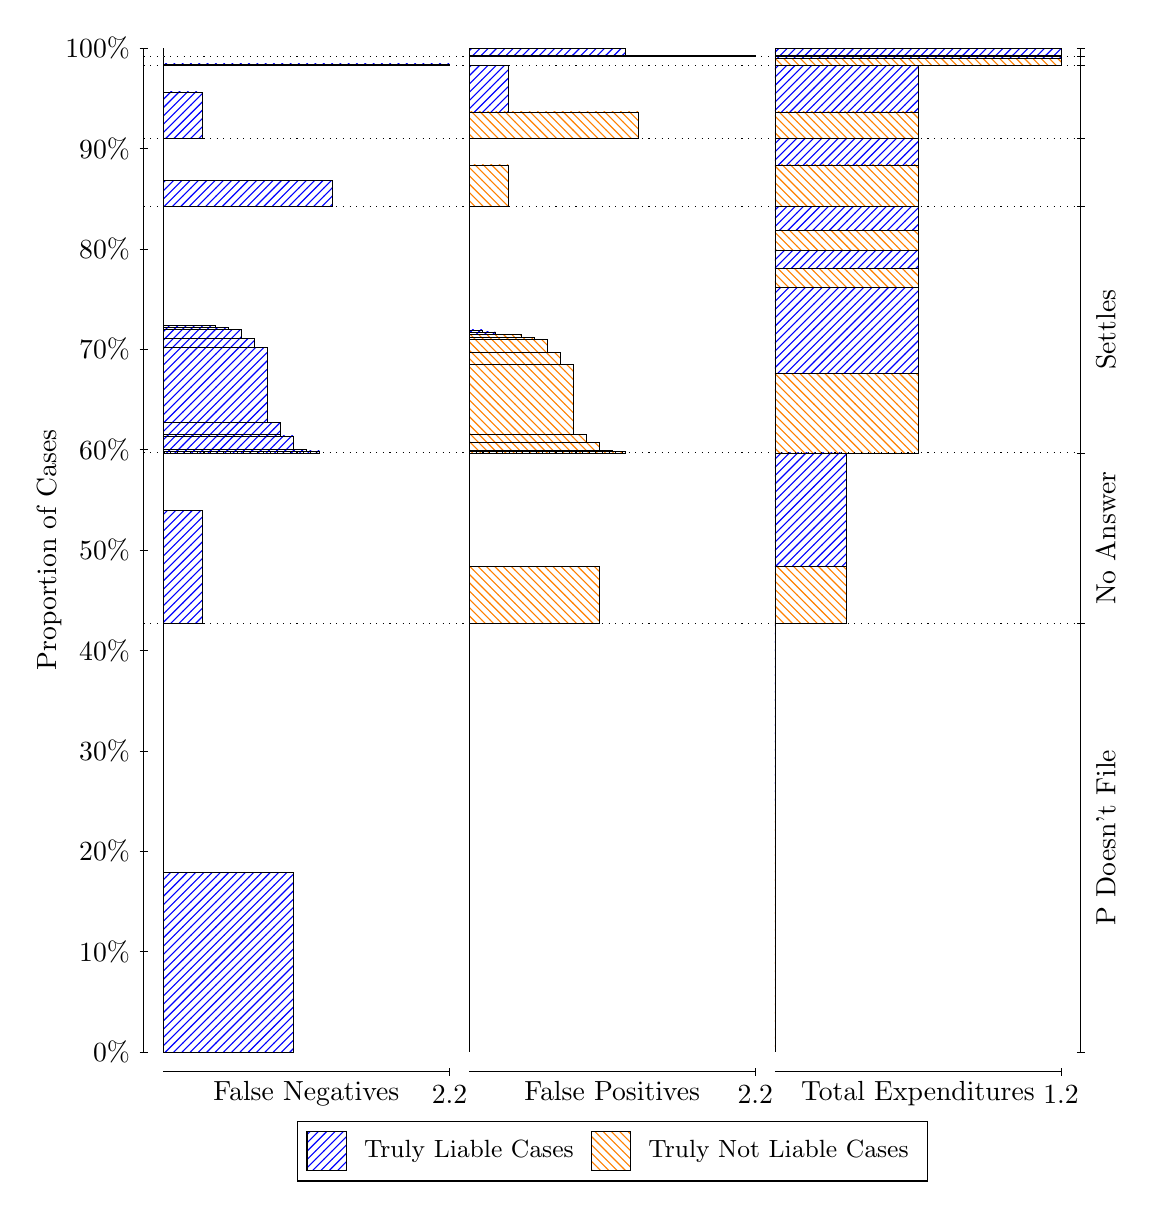
\begin{tikzpicture}
\draw[black, very thin] (1.5,1.75) -- (1.5,14.5);
\node[rotate=90, anchor=center] at (0.3, 8.125) {Proportion of Cases};
\draw[black, very thin] (1.45,1.75) -- (1.55,1.75);
\node[anchor=east] at (1.45, 1.75) {0\%};
\draw[black, very thin] (1.45,3.025) -- (1.55,3.025);
\node[anchor=east] at (1.45, 3.025) {10\%};
\draw[black, very thin] (1.45,4.3) -- (1.55,4.3);
\node[anchor=east] at (1.45, 4.3) {20\%};
\draw[black, very thin] (1.45,5.575) -- (1.55,5.575);
\node[anchor=east] at (1.45, 5.575) {30\%};
\draw[black, very thin] (1.45,6.85) -- (1.55,6.85);
\node[anchor=east] at (1.45, 6.85) {40\%};
\draw[black, very thin] (1.45,8.125) -- (1.55,8.125);
\node[anchor=east] at (1.45, 8.125) {50\%};
\draw[black, very thin] (1.45,9.4) -- (1.55,9.4);
\node[anchor=east] at (1.45, 9.4) {60\%};
\draw[black, very thin] (1.45,10.675) -- (1.55,10.675);
\node[anchor=east] at (1.45, 10.675) {70\%};
\draw[black, very thin] (1.45,11.95) -- (1.55,11.95);
\node[anchor=east] at (1.45, 11.95) {80\%};
\draw[black, very thin] (1.45,13.225) -- (1.55,13.225);
\node[anchor=east] at (1.45, 13.225) {90\%};
\draw[black, very thin] (1.45,14.5) -- (1.55,14.5);
\node[anchor=east] at (1.45, 14.5) {100\%};

\draw[black, very thin] (13.4,1.75) -- (13.4,14.5);
\draw[black, very thin] (13.35,1.75) -- (13.45,1.75);
\node[anchor=west] at (13.35, 1.75) {};
\draw[black, very thin] (13.35,7.1902) -- (13.45,7.1902);
\node[anchor=west] at (13.35, 7.1902) {};
\draw[black, very thin] (13.35,9.3597) -- (13.45,9.3597);
\node[anchor=west] at (13.35, 9.3597) {};
\draw[black, very thin] (13.35,12.484) -- (13.45,12.484);
\node[anchor=west] at (13.35, 12.484) {};
\draw[black, very thin] (13.35,13.354) -- (13.45,13.354);
\node[anchor=west] at (13.35, 13.354) {};
\draw[black, very thin] (13.35,14.28) -- (13.45,14.28);
\node[anchor=west] at (13.35, 14.28) {};
\draw[black, very thin] (13.35,14.391) -- (13.45,14.391);
\node[anchor=west] at (13.35, 14.391) {};
\draw[black, very thin] (13.35,14.5) -- (13.45,14.5);
\node[anchor=west] at (13.35, 14.5) {};

\draw[black, very thin, pattern color=blue, pattern=north east lines] (1.75,1.75) rectangle (3.4015,4.0306);
\draw[black, very thin, pattern color=orange, pattern=north west lines] (1.75,4.0306) rectangle (1.75,7.1902);
\draw[black, very thin, pattern color=blue, pattern=north east lines] (1.75,7.1902) rectangle (2.2455,8.6282);
\draw[black, very thin, pattern color=orange, pattern=north west lines] (1.75,8.6282) rectangle (1.75,9.3597);
\draw[black, very thin, pattern color=blue, pattern=north east lines] (1.75,9.3597) rectangle (3.7318,9.3824);
\draw[black, very thin, pattern color=blue, pattern=north east lines] (1.75,9.3824) rectangle (3.5667,9.4017);
\draw[black, very thin, pattern color=blue, pattern=north east lines] (1.75,9.4017) rectangle (3.4015,9.5746);
\draw[black, very thin, pattern color=blue, pattern=north east lines] (1.75,9.5746) rectangle (3.2364,9.5912);
\draw[black, very thin, pattern color=blue, pattern=north east lines] (1.75,9.5912) rectangle (3.2364,9.7444);
\draw[black, very thin, pattern color=blue, pattern=north east lines] (1.75,9.7444) rectangle (3.0712,10.698);
\draw[black, very thin, pattern color=blue, pattern=north east lines] (1.75,10.698) rectangle (2.9061,10.81);
\draw[black, very thin, pattern color=blue, pattern=north east lines] (1.75,10.81) rectangle (2.7409,10.923);
\draw[black, very thin, pattern color=blue, pattern=north east lines] (1.75,10.923) rectangle (2.5758,10.948);
\draw[black, very thin, pattern color=blue, pattern=north east lines] (1.75,10.948) rectangle (2.4106,10.978);
\draw[black, very thin, pattern color=orange, pattern=north west lines] (1.75,10.978) rectangle (1.75,12.484);
\draw[black, very thin, pattern color=blue, pattern=north east lines] (1.75,12.484) rectangle (3.897,12.823);
\draw[black, very thin, pattern color=orange, pattern=north west lines] (1.75,12.823) rectangle (1.75,13.354);
\draw[black, very thin, pattern color=blue, pattern=north east lines] (1.75,13.354) rectangle (2.2455,13.944);
\draw[black, very thin, pattern color=orange, pattern=north west lines] (1.75,13.944) rectangle (1.75,14.28);
\draw[black, very thin, pattern color=blue, pattern=north east lines] (1.75,14.28) rectangle (5.3833,14.299);
\draw[black, very thin, pattern color=orange, pattern=north west lines] (1.75,14.299) rectangle (1.75,14.391);
\draw[black, very thin, pattern color=orange, pattern=north west lines] (1.75,14.391) rectangle (1.75,14.41);
\draw[black, very thin, pattern color=blue, pattern=north east lines] (1.75,14.41) rectangle (1.75,14.5);
\draw[black, very thin, pattern color=orange, pattern=north west lines] (5.6333,1.75) rectangle (5.6333,4.9095);
\draw[black, very thin, pattern color=blue, pattern=north east lines] (5.6333,4.9095) rectangle (5.6333,7.1902);
\draw[black, very thin, pattern color=orange, pattern=north west lines] (5.6333,7.1902) rectangle (7.2848,7.9217);
\draw[black, very thin, pattern color=blue, pattern=north east lines] (5.6333,7.9217) rectangle (5.6333,9.3597);
\draw[black, very thin, pattern color=orange, pattern=north west lines] (5.6333,9.3597) rectangle (7.6152,9.3762);
\draw[black, very thin, pattern color=orange, pattern=north west lines] (5.6333,9.3762) rectangle (7.45,9.3917);
\draw[black, very thin, pattern color=orange, pattern=north west lines] (5.6333,9.3917) rectangle (7.2848,9.4908);
\draw[black, very thin, pattern color=orange, pattern=north west lines] (5.6333,9.4908) rectangle (7.1197,9.5899);
\draw[black, very thin, pattern color=orange, pattern=north west lines] (5.6333,9.5899) rectangle (6.9545,10.482);
\draw[black, very thin, pattern color=orange, pattern=north west lines] (5.6333,10.482) rectangle (6.7894,10.637);
\draw[black, very thin, pattern color=orange, pattern=north west lines] (5.6333,10.637) rectangle (6.6242,10.799);
\draw[black, very thin, pattern color=orange, pattern=north west lines] (5.6333,10.799) rectangle (6.4591,10.826);
\draw[black, very thin, pattern color=orange, pattern=north west lines] (5.6333,10.826) rectangle (6.2939,10.865);
\draw[black, very thin, pattern color=blue, pattern=north east lines] (5.6333,10.865) rectangle (5.9636,10.895);
\draw[black, very thin, pattern color=blue, pattern=north east lines] (5.6333,10.895) rectangle (5.7985,10.92);
\draw[black, very thin, pattern color=blue, pattern=north east lines] (5.6333,10.92) rectangle (5.6333,12.484);
\draw[black, very thin, pattern color=orange, pattern=north west lines] (5.6333,12.484) rectangle (6.1288,13.015);
\draw[black, very thin, pattern color=blue, pattern=north east lines] (5.6333,13.015) rectangle (5.6333,13.354);
\draw[black, very thin, pattern color=orange, pattern=north west lines] (5.6333,13.354) rectangle (7.7803,13.69);
\draw[black, very thin, pattern color=blue, pattern=north east lines] (5.6333,13.69) rectangle (6.1288,14.28);
\draw[black, very thin, pattern color=orange, pattern=north west lines] (5.6333,14.28) rectangle (5.6333,14.371);
\draw[black, very thin, pattern color=blue, pattern=north east lines] (5.6333,14.371) rectangle (5.6333,14.391);
\draw[black, very thin, pattern color=orange, pattern=north west lines] (5.6333,14.391) rectangle (9.2667,14.41);
\draw[black, very thin, pattern color=blue, pattern=north east lines] (5.6333,14.41) rectangle (7.6152,14.5);
\draw[black, very thin, pattern color=orange, pattern=north west lines] (9.5167,1.75) rectangle (9.5167,4.9095);
\draw[black, very thin, pattern color=blue, pattern=north east lines] (9.5167,4.9095) rectangle (9.5167,7.1902);
\draw[black, very thin, pattern color=orange, pattern=north west lines] (9.5167,7.1902) rectangle (10.425,7.9217);
\draw[black, very thin, pattern color=blue, pattern=north east lines] (9.5167,7.9217) rectangle (10.425,9.3597);
\draw[black, very thin, pattern color=orange, pattern=north west lines] (9.5167,9.3597) rectangle (11.333,10.366);
\draw[black, very thin, pattern color=blue, pattern=north east lines] (9.5167,10.366) rectangle (11.333,11.458);
\draw[black, very thin, pattern color=orange, pattern=north west lines] (9.5167,11.458) rectangle (11.333,11.699);
\draw[black, very thin, pattern color=blue, pattern=north east lines] (9.5167,11.699) rectangle (11.333,11.931);
\draw[black, very thin, pattern color=orange, pattern=north west lines] (9.5167,11.931) rectangle (11.333,12.189);
\draw[black, very thin, pattern color=blue, pattern=north east lines] (9.5167,12.189) rectangle (11.333,12.484);
\draw[black, very thin, pattern color=orange, pattern=north west lines] (9.5167,12.484) rectangle (11.333,13.015);
\draw[black, very thin, pattern color=blue, pattern=north east lines] (9.5167,13.015) rectangle (11.333,13.354);
\draw[black, very thin, pattern color=orange, pattern=north west lines] (9.5167,13.354) rectangle (11.333,13.69);
\draw[black, very thin, pattern color=blue, pattern=north east lines] (9.5167,13.69) rectangle (11.333,14.28);
\draw[black, very thin, pattern color=orange, pattern=north west lines] (9.5167,14.28) rectangle (13.15,14.371);
\draw[black, very thin, pattern color=blue, pattern=north east lines] (9.5167,14.371) rectangle (13.15,14.391);
\draw[black, very thin, pattern color=orange, pattern=north west lines] (9.5167,14.391) rectangle (13.15,14.41);
\draw[black, very thin, pattern color=blue, pattern=north east lines] (9.5167,14.41) rectangle (13.15,14.5);
\draw[black, dotted] (1.5,7.1902) -- (13.4,7.1902);
\draw[black, dotted] (1.5,9.3597) -- (13.4,9.3597);
\draw[black, dotted] (1.5,12.484) -- (13.4,12.484);
\draw[black, dotted] (1.5,13.354) -- (13.4,13.354);
\draw[black, dotted] (1.5,14.28) -- (13.4,14.28);
\draw[black, dotted] (1.5,14.391) -- (13.4,14.391);
\draw[black, very thin] (1.75,1.5) -- (5.3833,1.5);
\node[anchor=north] at (3.5667, 1.5) {False Negatives};
\draw[black, very thin] (5.3833,1.45) -- (5.3833,1.55);
\node[anchor=north] at (5.3833, 1.45) {2.2};

\draw[black, very thin] (5.6333,1.5) -- (9.2667,1.5);
\node[anchor=north] at (7.45, 1.5) {False Positives};
\draw[black, very thin] (9.2667,1.45) -- (9.2667,1.55);
\node[anchor=north] at (9.2667, 1.45) {2.2};

\draw[black, very thin] (9.5167,1.5) -- (13.15,1.5);
\node[anchor=north] at (11.333, 1.5) {Total Expenditures};
\draw[black, very thin] (13.15,1.45) -- (13.15,1.55);
\node[anchor=north] at (13.15, 1.45) {1.2};

\node[black, centered, rotate=90] at (13.72, 4.4701) {P Doesn't File};
\node[black, centered, rotate=90] at (13.72, 8.2749) {No Answer};
\node[black, centered, rotate=90] at (13.72, 10.922) {Settles};





\draw (7.449999999999999,1.5) node[draw=none] (baseCoordinate) {};
\begin{scope}[align=center]
        \matrix[scale=0.5, draw=black, below=0.5cm of baseCoordinate, nodes={draw}, column sep=0.1cm]{
            \node[rectangle, draw, minimum width=0.5cm, minimum height=0.5cm, pattern=north east lines, pattern color=blue] {}; &
            \node[draw=none, font=\small] (B) {Truly Liable Cases}; &
            \node[rectangle, draw, minimum width=0.5cm, minimum height=0.5cm, pattern=north west lines, pattern color=orange] {}; &
            \node[draw=none, font=\small] (B) {Truly Not Liable Cases}; \\
            };
\end{scope}

\end{tikzpicture}
\end{document}